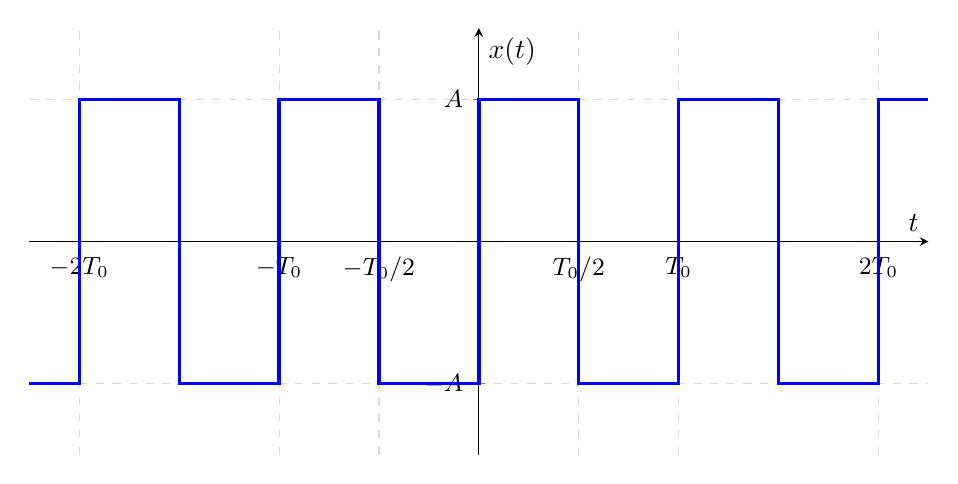
\begin{tikzpicture}
\begin{axis}[
    width=13cm, 
    height=7cm,
    axis lines=middle,
    xlabel={$t$},
    ylabel={$x(t)$},
    xmin=-4.5, 
    xmax=4.5,
    ymin=-1.5, 
    ymax=1.5,
    xtick={-4, -2, -1, 1, 2, 4},
    xticklabels={$-2T_0$, $-T_0$, $-T_0/2$, $T_0/2$, $T_0$, $2T_0$},
    ytick={-1, 1},
    yticklabels={$-A$, $A$},
    grid=both,
    grid style={dashed, gray!30},
    tick label style={font=\small},
    clip=false
]

% Draw the square wave using simple lines
\draw[blue, very thick] 
    (axis cs:-4.5, -1) -- (axis cs:-4, -1) -- (axis cs:-4, 1) -- (axis cs:-3, 1) 
    -- (axis cs:-3, -1) -- (axis cs:-2, -1) -- (axis cs:-2, 1) -- (axis cs:-1, 1)
    -- (axis cs:-1, -1) -- (axis cs:0, -1) -- (axis cs:0, 1) -- (axis cs:1, 1)
    -- (axis cs:1, -1) -- (axis cs:2, -1) -- (axis cs:2, 1) -- (axis cs:3, 1)
    -- (axis cs:3, -1) -- (axis cs:4, -1) -- (axis cs:4, 1) -- (axis cs:4.5, 1);

\end{axis}
\end{tikzpicture}